\chapter{State of the Art}
\label{chapter:state_of_the_art}

% TODO
% - check https://repository.kaust.edu.sa/handle/10754/673882
% - acabar de rever os paragrafos dos artigos

\section{Background Material}

\subsection{Anticipation in Biology}

 Anticipating actions is an idea that comes from biology, given that humans and many other animals anticipate each other constantly. In biology research, we can find a definition such as the one stated in \cite{Rosen1985}: "An anticipatory system is a system containing a predictive model of itself and/or its environment, which allows it to change state at an instant in accord with the model's predictions pertaining to a later instant.".

\subsection{Machine Learning}

Machine Learning algorithms have been increasingly more common in the last years due to, for example, their ability to deal with multidimensional data. These algorithms can automatically learn from data and make predictions or decisions, which makes them a prime candidate to use in the context of human action anticipation in collaborative environments. The most common strategies in this field are Supervised Learning, Unsupervised Learning, and Reinforcement Learning. As we can see in Fig.~\ref{machinelearning} obtained from a review article about HRC in general, supervised learning and reinforcement learning are dominant in this area, with composite solutions surpassing unsupervised learning in the most recent year showed.

\begin{figure}[H]
\centerline{\includegraphics[width=6in]{figs/machinelearning.PNG}}
\caption{Number of articles relevant to the HRC review from each machine learning technique throughout the years\cite{Semeraro2023}}
\label{machinelearning}
\end{figure}

\subsubsection{Supervised Learning}

In Supervised Learning, the models are trained using a dataset of labeled data. The models from this group are further divided into classification, where the new instance is assigned a particular class, and Regression, where it is given a certain real number. These models must generalize the knowledge from the examples to deal with a new instance correctly that they have never seen before. Among these models, convolutional and recurrent neural networks are at the forefront of the algorithms to explore.

A Recurrent Neural Network (RNN) is a type of neural network where the output of each time step is fed back into the input at the next time step, allowing the network to remember and incorporate information from previous time steps into its processing of current and future data. This characteristic makes RNNs particularly well-suited to processing sequential data, such as text, speech, or time series data which require context or temporal dependencies. In particular, LSTM is an RNN with a more complex architecture that gives it an improved ability to backpropagate the error, making it better to train a model that classifies sequences with several time steps.

A Convolutional Neural Network (CNN) is a type of neural network made up of several convolutional layers which apply a sliding filter over the input reducing its dimension and obtaining its features. Typically, these layers are followed by one or more fully connected layers that perform the prediction using the mentioned features. This architecture makes CNNs an excellent choice to deal with data in a matrix structure such as an image because this input is too massive for manual feature engineering.


\subsubsection{Unsupervised Learning}

In Unsupervised Learning, the datasets involved have no labels; therefore, the algorithms aim to find patterns and relationships in the data. This makes them valuable for finding structure in the data, creating clusters based on common characteristics, or identifying anomalies and outliers.

\subsubsection{Reinforcement Learning}

In Reinforcement Learning, the model is trained to decide which action to take in a specific environment to maximize a particular reward function. These algorithms learn through trial and error using the reward they obtain in each iteration to improve their performance continuously. This type of learning has a certain resemblance to how humans gain knowledge, and it is useful when there is a need for an agent to make decisions in an environment that has considerable complexity, such as controlling a robot or playing a game.

\subsubsection{Transfer Learning}

Since most work uses images as input, transfer learning is also common in the literature. This type of learning involves using a neural network, usually convolutional, that was pre-trained in another dataset. Depending on the goal of its use, these networks can be used entirely or partially; optionally, they can also be trained partially or fully. Some of the most popular examples include VGG-16 and ResNet-50.

\subsection{Collaborative Robotics}

In Human-Robot Collaboration there is a need to use robots different from the classic industrial ones given that they will be working in the same workspace as humans. To achieve this, Collaborative Robots or Cobots have been developed with significant advantages when working with people. For once, they can safely work with people since they have sensitive sensors that can detect the human interrupting them, causing them to stop their actions. They are also smaller, compact, and easy to program, among other advantages. \cite{CobotsWW}

In Fig.~\ref{interaction}, we can see a diagram containing multiple data sources that can be used to implement communication between the robot and the human, along with its advantages and disadvantages.

\begin{figure}[H]
\centerline{\includegraphics[width=6in]{figs/interaction.PNG}}
\caption{Advantages and Disadvantages of some Data Sources in Human-Robot Collaboration \cite{Mukherjee2022}}
\label{interaction}
\end{figure}

\subsubsection{Gestures}

Gestures are one of the main ways humans communicate with each other whether through simple movements or formal sign language. In work about Human-Robot Collaboration, gestures can also commonly be found since it has the advantage of resisting ambient noise.

Usually, gestures are captured with vision-based methods with either an RGB or RGB-D camera, so there is no need for unnatural movements. With vision, it is possible to include markers but these may lead to occlusions and hinder the worker's movements. Consequently, there is also work that uses markerless vision to allow more unrestricted movements.

Another way to capture the movements of the human worker would be to use wearable inertial sensors, which contain accelerometers and gyroscopes, but, once again, wearables can hinder the worker's movements.

\subsubsection{Natural Language}

Natural Language is the main and the most intuitive way for humans to communicate with each other. The advances in natural language processing make this a possible solution for communication with robots too. However, despite being intuitive, simple, effective, and even robust against lighting variations, when it comes to an industrial setting that contains significant sound noise, it becomes less valuable than the alternatives.

\subsubsection{Gaze}

Next, the gaze can also be used to determine where the user's attention resides, which gives a considerable amount of information that can be used to trigger some action.

There are two options to obtain the user's gaze. Wearable sensors can provide better results but are expensive and intrusive. On the other hand, algorithms that detect head pose and assume the gaze from it can also be used, which is a cheaper and non-intrusive solution.

\subsubsection{Emotions through Facial Expressions}

Although this is a relatively new idea, some applications analyze the user's emotions from his facial expressions to have even more information in the algorithms.

\subsubsection{Semantics}

Finally, semantic information about the objects can also help the global workflow. For example, suppose the robot is trained to recognize certain features in objects related to how it can pick them up. In this case, the robot can pick up a new object it has never seen before if it has a similar structure.

Human actions can also be represented semantically by obtaining the poses of the human as a specific set of limbs, even if only partially. During action recognition, this can be used to know which objects the worker can interact with.

Having information about the pose of the human body also helps in the path-planning phase of the robot since it can use this information to avoid the worker and prevent collisions.

{\color{red} maybe put some text about biometric sensors}

\section{Data Sources and Sensors}

The first step to anticipating the following action is to know what kind of data we should collect with the sensors. Previously, several forms of communication between the human and the robot were described. Still, these work in a more active way and not all of them can be applied to action anticipation where the user should not need to do anything for the robot to act. Essentially, there is a need to capture the human's body language.

As humans usually anticipate each other by poses and gestures, these factors became some of the most common data to perform action anticipation. Regarding sensors, most of the literature suggests using an RGB camera. Still, some works, such as the one described in \cite{Moutinho2023}, indicate the use of an RGB-D camera to capture both the color and the depth images. If wearable sensors are an option, inertial sensors also become an alternative.

In \cite{Maeda2016} the authors also used markers to obtain the gestures of the human.

In \cite{Gammulle2019}, \cite{Wu2021}, \cite{Rodriguez2019}, and \cite{Furnari2021}, the authors went a step further and used the images but also processed the optical flow between them and used it in their algorithms.

In \cite{Canuto2021}, the authors used OpenPose\footnote{OpenPose documentation:

https://cmu-perceptual-computing-lab.github.io/openpose}\cite{Cao2021}\cite{Simon2017}\cite{Cao2018}\cite{Wei2016} which is a framework with pre-trained models that receive an image, process it, and return 3D points representing the skeleton joints of the person in the image, as we can see in Fig.~\ref{openpose}.

\begin{figure}[H]
\centerline{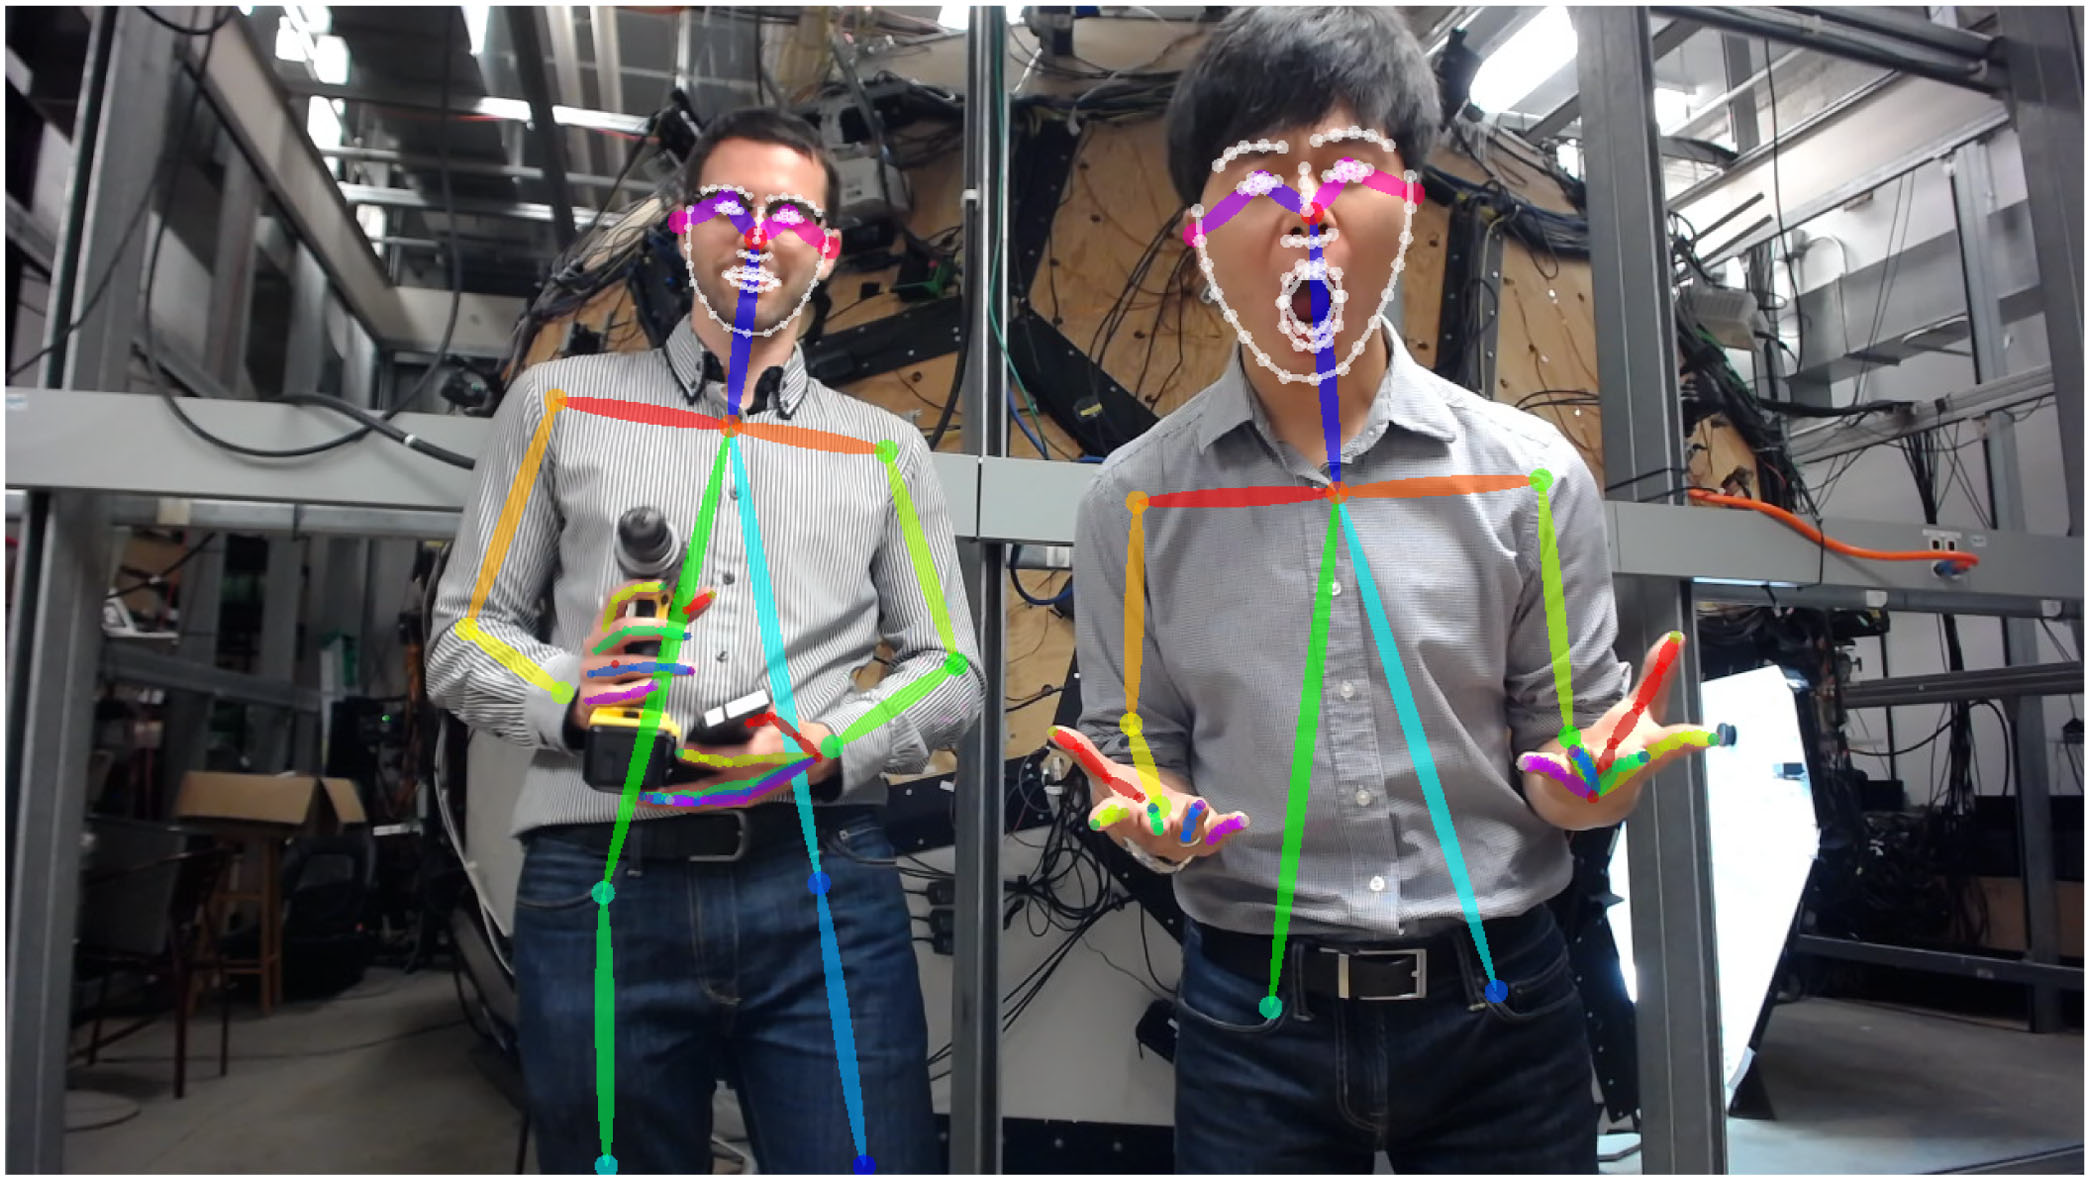
\includegraphics[width=3.5in]{figs/openpose.PNG}}
\caption{OpenPose example\cite{Cao2021}}
\label{openpose}
\end{figure}

Humans also tend to anticipate each other by considering the other's gaze, which usually indicates his center of attention. As this is also an involuntary aspect, there is some work where gaze provides additional information, such as in \cite{Schydlo2018} where the dataset contained the gaze of the user captured with wearable sensors or in \cite{Canuto2021} where the gaze was assumed from the results of an algorithm to detect the head pose.

In addition to the data related to the human, the objects present in the environment can also give valuable information about the human's following action, as is the case in \cite{Furnari2021}.

\section{Algorithms}

After knowing which is usually captured and provided to an algorithm, this section explores possible algorithmic solutions present in previous work.

\subsection{Supervised Learning Solutions}

The aim of this thesis can be represented as a Classification problem since it is possible to use a sequence of images that must be classified as a particular future action class. Using Fig.~\ref{superviseddiagram} as an example, the high-five action should be predicted before the frames that contain it are captured. The previous work with this kind of algorithm mainly includes convolutional and recurrent neural networks, with the latter being the most common.

\begin{figure}[H]
\centerline{\includegraphics[width=3.5in]{figs/superviseddiagram.PNG}}
\caption{Action Anticipation using Supervised Learning diagram\cite{Gammulle2019}}
\label{superviseddiagram}
\end{figure}

% LSTM only examples
In \cite{Canuto2021}, the authors aimed to predict the following action using a Long Short-Term Memory (LSTM) neural network, one of the most common RNNs. In their work, they used a dataset captured with an RGB camera. From these images, they obtained the objects in the environment, the human skeleton joints extracted over time using OpenPose, and the gaze derived from the joints. Then the three data sources were given to the LSTM as input to perform the desired classification. In this process, the authors use an adaptive threshold on the uncertainty of the recurrent neural network, which makes the model need a certain level of certainty to classify the action as a particular class. This creates a more robust solution since a standard supervised learning algorithm would predict the class with the highest probability even if the model has low certainty about every category.

In \cite{Furnari2021}, the authors aimed to predict the subsequent actions that someone wearing a camera would perform and the objects he would interact with. They used three datasets containing RBG frames from which they derived the optical flow and the things in the environment. This data is then passed on to a Rolling-Unrolling LSTM. The Rolling LSTM (R-LSTM) is a network that continuously encodes the received observations and keeps an updated summary of the past. When it is time to make predictions about future actions, the Unrolling LSTM (U-LSTM) is used with its hidden and cell states equal to the current ones of the R-LSTM.

In \cite{Schydlo2018}, the authors used an encoder-decoder recurrent neural network topology to predict human actions and intent where the encoder and the decoder are both LSTM cells. At each step, the decoder returns a discrete distribution of the possible actions making this algorithm able to consider multiple action sequences, which are then subject to a pruning method that reduces them to obtain the right action finally. In their work, these algorithms were tested in two different datasets, one containing RGB images with optical markers and gaze information from wearable sensors and another with RGB-D images.

% LSTM + CNN
In \cite{Zhang2022}, the authors aimed to predict the intention of the human worker to provide him with the required piece. To achieve this, they used an RGB camera to capture the data from the environment. Then the images are given to a convLSTM framework where the CNN part is in charge of extracting features from the input images, and these features are then passed on to the LSTM to predict the intention. Additionally, another CNN is in charge of recognizing the required piece when the robot is fetching it. This article also tackles the issue of having several possible assembly orders. It solves it by creating a phase at the beginning of the collaboration in which the robot learns the assembly actions and their order from a demonstration.

% ResNet-34 + LSTM
In \cite{Moutinho2023}, the authors aimed to increase the natural collaboration between the robot and the human in an assembly station by interpreting implicit communication cues. The data related to the environment was captured using an RGB-D camera. This data was then passed on to a ResNet-34, a pre-trained neural network that extracted the features from the images. These features are used as the input to an LSTM to perform human action recognition.

% ResNet-50 + LSTM
In \cite{Gammulle2019}, the authors aimed to predict future frames while at the same time predicting the following action. In their implementation, they used public datasets with videos from which they obtained RGB images and optical flow streams. To consider both sources of data, they also used two ResNet-50's, which are pre-trained networks, one to get the input features from the image and another from the optical flow, and 2 LSTMs to take into account both sequences of inputs. Then the two results are merged into a final classification. They also used two Generative Adversarial Networks (GAN) to generate the subsequent frames, but this is different from the focus of the analysis.

% double % might need rework
%% VGG-16 + TTM
In \cite{Wang2021}, the authors used video datasets to train a model that would predict a future action from the observed frames. They used three pre-trained neural networks in their work: VGG-16, TS, and ConvNet, to extract features from the images. Then these features were aggregated using a Temporal Transformer module (TTM), and finally, a progressive prediction module (PPM) would anticipate the worker's future action. This article also addresses the issue of specifying what the algorithm should consider as an action. Although most of the literature often implies that the last frames captured by the camera are considered an action, given that those are the frames that contain the last action made by the user, the authors of this article go into greater detail. They tested and evaluated how many frames should be considered as the last action to obtain the best results using a metric from \cite{Geest2016} named per-frame calibrated average precision (cAP) calculated with \eqref{eq}. In \cite{Wang2021} it is defined with

\begin{equation}
cAP=\frac{\sum_k cPrec(k) * I(k)}{P},
\label{eq}
\end{equation}

"where  calibrated  precision $cPrec=\frac{TP}{TP+FP/w}$, $I(k)$ is an indicator function that is equal to 1 if the cut-off frame k is a true positive, $P$ denotes the total number of true positives, and $w$ is the ratio between negative and positive frames. The mean cAP over all classes is reported for final performance.".

%% CNN
In \cite{Rodriguez2019}, the authors aimed to predict the following action by first predicting the following motion images. They used datasets containing videos and then processed them to obtain motion images. These motion images become the input of a convolutional autoencoder network that generates the following motion images. These images are then passed to a Convolutional Neural Network (CNN) that processes them and makes action predictions for the future. The final action prediction is obtained from the results of the previous network and those of a second CNN, which analyzes the original RGB images.

%% architecture with TSN (very complex overall)
In \cite{Wu2021}, the author's goal was to predict the following action someone wearing a camera would perform after some time. Initially, the optical flow was obtained from the captured images, and both were used as input to the model. The model is comprised of a Temporal Segment Networks (TSN), a CNN, and an LSTM to predict the future frame features and then use them to perform the required classification.

% Look-up table
Apart from deep learning, there are also more classical approaches such as \cite{Maeda2016}, where the authors aimed to reduce the delay in the robot's response by predicting the human worker and providing a screw or a plate accordingly. They captured the environment using an RGB camera and tracked the hand using optical markers. Then they predicted the following human action using a look-up table containing different orders for assembly actions. With the nearest neighbor algorithm, the actions of the human would be matched with a particular order. If the robot eventually notices that it did the wrong action, it would then follow a hard-coded contingency trajectory to return to the pre-grasping position. The limitation of this method is that all possible sequences need to be on the table because if they are not there, then the robot will match with a different order which may be undesirable.

{\color{red}
\subsection{Unsupervised Learning Solutions(possibly to delete)}

In \cite{Kato2018}, the authors attempted to recognize human actions using the trajectories of skeleton joints. The environment was captured using a RGB camera and then the joints were obtained using OpenPose.
}

{\color{red} explain the rest of the model}

\subsection{Reinforcement Learning Solutions}

% POMDP
In \cite{Gorur2018}, the authors aimed to make the human-robot interaction more natural by detecting unexpected conditions where the human will not need the robot's assistance, such as when the human's current intention is unknown or irrelevant to the robot or when even though the human's intent is relevant, that task is done only by the human. They used the algorithm Partially Observable Markov Decision Process (POMDP) to achieve this. The training was done with simulation with the model learning a policy by having a positive reward if the task was accomplished and a negative reward if the robot tried to help the human in a situation where it should not.

\section{Human-Robot Collaboration Safety}

Finally, safety is a topic that must always be mentioned when robots work with humans, especially in human-robot collaboration. Although collaborative robots or cobots nowadays are made so that if they are interrupted in their work, they switch to a safety mode, effectively stopping, they are still machines with significant strength and can potentially harm the user.

Firstly, just anticipating the actions of the human worker is already a safety measure since it increases the robot's ability to avoid collisions.

In \cite{Zhang2022}, the authors defined speed limits on the robot and ensured that the robot would avoid the workspace of the human. Then when it needs to move closer to the user, its speed is reduced to guarantee the user's safety.

In \cite{Wu2023}, the authors used deep deterministic policy gradient (DDPG) to plan the robot's trajectory so that the robot would not collide with the human to guarantee his safety.

In \cite{Psarakis2022}, the authors attempted to create a sense of anticipation in humans towards the robot's movements through visual cues of the robot's upcoming action, which is the reverse of what it is being tried to achieve in the other reviewed papers. As with the previous article, they also made it so the robot must reduce its movement speed when close to the robot. Although it was only tested in the Virtual Reality simulation shown in Fig.~\ref{vr}, where the users feel safer, they concluded that the efficiency of the collaboration was increased, and the user had a greater feeling of safety and trust. Furthermore, knowing what the robot will do next also decreases the risk of a collision since the user will avoid the space where the robot is working, increasing safety.

\begin{figure}[H]
\centerline{\includegraphics[width=3.5in]{figs/reverse.PNG}}
\caption{VR Simulation of \cite{Psarakis2022}, the orange means the robot will pick that puck next}
\label{vr}
\end{figure}

In \cite{Mukherjee2022}, it is also referred that limiting the power and force of the robot decreases the gravity of the consequences of a possible collision, increasing safety. Nowadays, this feature is already included in collaborative robots.